\chapter{Evaluation}\label{s:evaluation}

\section{Design of experiment}
This research is based on a theory stating privacy breaches of citizens are a growing issue and technologies could be applied more broadly to mitigate this issue. Scope of these issues seemed to be clear in the design phase of the experiment. However, after discussing the experiment subject with consulted experts the view on a UIN as a secluded problem and techniques of tokenization and pseudonymization as a set of viable possible solution seemed too narrow. Resulting in different research scope and broader literature study to define the operational problem. Practical understanding of problems, goals and solutions was gathered via semi-structured interviews with experts in the field of governmental identity data.

\section{Methodology}
Research method is approached as an inductive exploratory experiment based on the theory technologies could support privacy preservation of citizens. Understanding the possible problems was part of this research therefore being an interpretive research.

Experts where consulted in bringing focus to the research problem and scope. These consulted experts referred to available literature and therefore these conversations where not recorded and transcribed. To get a more detailed view and problem definition semi-structured interviews where conducted with experts. Interviews are in Dutch and therefore transcription is in Dutch. Information is extracted by using the coding method and translated in English during this process. Williams and Moser \cite{Williams2019TheAO} claim: "Regardless of the research approach, the methodology employed for data collection and
organization must be clear and repeatable, leading to and enabling data analysis..... A key data organizing structure in qualitative research is coding." This is why coding method has been used. 

    \begin{figure}
        \graphicspath{ {./images/} }
        \centering
        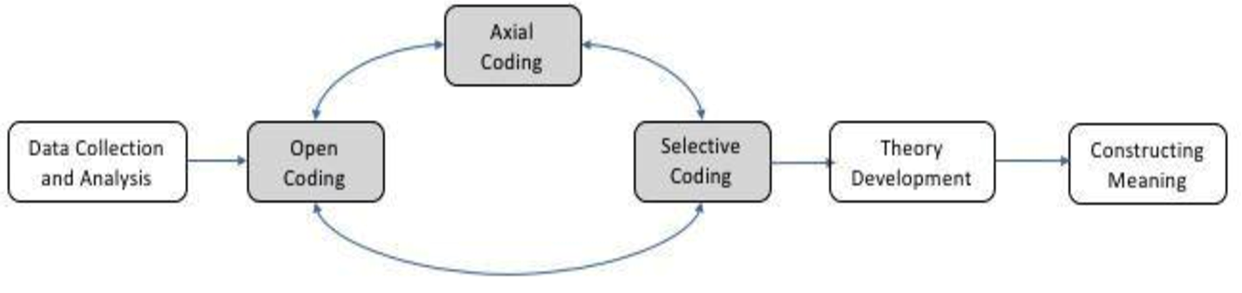
\includegraphics[width=14cm]{Williams and Moser.png}\\
        \caption{Non-Linear Process. Williams and Moser \cite{Williams2019TheAO}}
        \label{fig:WM2019}
    \end{figure}

Transcribing the interviews is part of the "Data collection and Analysis" phase. "Open coding" has been done by marking possible interesting parts withing transcripts based on the themes of Business Goals and Concerns. The step of "Axial coding" results in refinement to Quality attributes defined by ISO-25010 \cite{ISO:25010:2011}. Quality Attributes considered to be Architecturally Significant refinements are defined in the last part of "Selective Coding". The phase of "Theory Development" and "Constructing Meaning" result in a utility tree with Attribute refinements and Quality Attribute scenarios. The output of this research is not a theory but a branch of Quality attributes divided into segments of solutions in the form of Quality attribute refinements.  Section \ref{s:overview} contains the Utility tree to depict the cohesion between these steps. In this way coding has been applied on methodology described in Software Architecture in Practice of Bass\etal \cite{Bass2015SoftwareAI}.

Biases will be discussed in Section \ref{sec:threats} 'Threats to validity'.

\section{Obtained results}
Themes in the form of Business Goals and Concerns are included in Appendix \ref{Appendix B} and Appendix \ref{Appendix C}. The results of translating them to Quality Attributes and Attribute Refinements in Figure \ref{fig:ASR1} combining them with the Business Goals and Concerns in Table \ref{ASR_BG_C}.



%\todo{
%Discuss the design of your experiments, the results you obtained, and how they
%help in evaluating the claims you made in the introduction. You may also use the
%evaluation results in this section to justify your design choices or assess the
%contributions of different aspects  of your design towards the overall goals.
%}

